%!TEX root = ThesisLKN.tex

\chapter{Implementation Details} \label{chapter:4}

In this chapter, the details on implementations will be described. In detail, how the ground truth data used for training network are generated from simulated human trajectories is described in Section \ref{sec:traj_sim}. In Section \ref{sec:training}, the details on training CNNs are provided. Section \ref{sec:BOFMP_implementation} introduces the code structure of implementing BOFMP. Finally, hyperparameters in the BOFMP tracking algorithm are introduced in Section \ref{sec:hyperparameter}.

\section{Human Trajectory Simulation} \label{sec:traj_sim}

Neural networks are able to capture complex structures in data. For this reason, we train a neural network so that it can be used to extract human motion patterns from static maps. In order to make the network generalizes well, a large amount of human trajectory data in different indoor environments are needed. However, recording human trajectories with 2D laser scans in various indoor environments is expensive, since the hardwares have to be transported to different locations. Besides, since our model requires cell-specific motion patterns, the recorded human trajectories need to cover each discretized cell on the gird map. Even if it is feasible, this requires a lot of time for the laser scanner to work. To collect such a huge amount of real human trajectories is obviously out of the scope of this thesis. As a workaround, we simulated human trajectories on real-world SLAM-generated maps and those simulated trajectories are used for extracting human motion patterns. To validate our method, we evaluate our tracking algorithm on data recorded from real world. 

The maps on which human trajectories are sampled from are floor plans of indoor environments such as laboratories and offices. We assume that human motions in these environment are only constrained by the spatial configurations. Other factors, such as time, social forces and different functional areas, are not modeled. In total, we simulate human trajectories on eight maps, with a total free space area of more than \( 6.6\times10^3 \, m^2 \). Two of those eight maps are shown in Figure \ref{fig:maps}. Each pixed of the map represents a cell on its corresponding occupancy grid, and has resolution of $0.2$ $m/pixel$.

\begin{figure}[ht]
  \centering
    
\includegraphics[width=.8\textwidth, height=.3\textwidth]{figures/map1.png}
    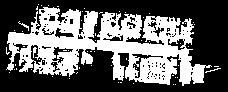
\includegraphics[width=.8\textwidth, height=.3\textwidth]{figures/map2.png}
    \caption[Two example maps on which human trajectories are sampled from.]{Two example maps on which human trajectories are sampled from. White areas are walkable, and black areas are desks or walls that human cannot walk through.}
    \label{fig:maps}
\end{figure} 

We use A* algorithm to calculate human trajectory between two points on a map. The A* algorithm is a well-know algorithm for path planning. In each iteration of its main loop, A* algorithm decides which step to take based on the summation of two values: one value represents the cost from start to current node and the other represents a heuristic estimate of cost from current node to the goal. The path found by A* algorithm replicates human trajectory, since people normally have a clear goal location in their mind (thus a heuristic estimation) and take a path that requires least efforts to reach it. To account for the fact that human tend to walk some distances away from an obstacle (e.g., people walk in the middle areas of a corridor, which are distant to walls on both sides), we apply two Gaussian filters with different widths on the static maps to get cost maps.  

The actual process from sampling trajectories to obtaining conditional probabilities as motion patterns are implemented in three steps:

\begin{my_enumerate}
\item Sampling trajectories on the full map. In order to get motion dynamics at all possible locations, we sample a predefined number of trajectories with every empty cell on the map as start location. The goal location for each trajectory is randomly sampled but the distance between start location and end location must be within a predefined range. After the start and goal location are defined, a trajectory is calculated by A* algorithm.
\item Calculate probabilities based on trajectories. A \textit{transition} is defined in this context as a person moves from cell $a$ to $c$ through $b$, i.e., $a \rightarrow b \rightarrow c$, where $a$ and $c$ are neighboring cells of $b$. If we consider eight neighboring cells, for each cell it has $8\times8=64$ different transitions. A helper function $v(c_1,c_2)$ is also defined to calculate the velocity from cell $c_1$ to $c_2$. Assume a cell $c$ is identified by its coordinates on $x$, $y$ axis, i.e, $pos(c)=(c_x, c_y)$, then
\[v(c_1, c_2)=\frac{pos(c_2)-pos(c_1)}{\Delta t}\]
Firstly a tensor $C$ is initialized to store these transition counts. So far, Tensor $C$ has 6 dimension of $32\times32\times3\times3\times3\times3$, with first two dimensions representing spatial size of a map window, next two dimensions representing $V^{en}$ and last two dimensions representing $V^{ex}$. For example, for transition $a \rightarrow b \rightarrow c$, we increment the following entry of $C$:
\[ C(pos(b), v(a, b), v(b, c))\]
For each sampled trajectory, we add every transition along this trajectory to its corresponding entry in $C$. The conditional probability $P_i(V^{ex}|V^{en})$ is then calculated from transition counts tensor $C$ as:
\begin{equation}
P_i(V^{ex}=v_1|V^{en}=v_0) = \frac{C(pos(i), v_0, v_1)}{\sum_{ v}C(pos(i), v_0, v)}
\end{equation}
\item Sampling map window with fixed size and data augmentation. The map window that we feed into our network is of size $32\times32$ cells (i.e., $6.4 \times 6.4$m). Therefore, we randomly crop a predefined number of map windows from the whole map. If a map window has free space less than $50\%$, it is not used. To increase the number of data samples, each map window is augmented eight times: for both the map window and its horizontal mirroring, they are rotated by $90^\circ$, $180^\circ$ and $270^\circ$. 

  So far, the ground truth of each map window has same dimensions as $C$, i.e, $32\times32\times3\times3\times3\times3$. However, since the output of network has at most three dimensions, the ground truth has to be resized to $32\times32\times64$, without considering velocity $v=(0, 0)$.
\end{my_enumerate}

The above algorithm is described in Algorithm \ref{algo:data_generation}. 

\begin{algorithm}
\caption{Algorithm for generating data for neural network.}
\label{algo:data_generation}
\begin{algorithmic}[1]
\Procedure{SamplingTrajectories(map, n)}{}
\State $allTrajectories \gets \emptyset$
\For{\textit{cell} in \textit{emptyCells(map)}} 
    \Comment loop over all empty cells on map
	\State $trajectories \gets \emptyset $
	\State $tries \gets 0$
	\While{$tries < N $} 
	\Comment try to sample $N$ trajectories for each cell
	\State $start \gets cell$
	\State $goal \gets sampleGoalLocation(map, start)$
	\State $trajectory \gets AStar(start, goal)$
	\If {$isValid(trajectory)$} 
		\Comment check whether $trajectory$ is empty
		\State \textbf{add} $trajectory$ \textbf{to} $trajectories$
	\EndIf
	\State $tries \gets tries+1$
	\EndWhile
	\State \textbf{append} $trajectories$ \textbf{to} $allTrajectories$
\EndFor
\State \Return $allTrajectories$
\EndProcedure
\\
\Procedure{GetConditionalProbs(Trajectories)}{}
\State Initialize $C$ with zeros
\For{\textit{trajectory} $(c_1, \cdots, c_n)$ in \textit{trajectories}} 
    \Comment loop over all sampled trajectories
    \For{$t=2:n-1$}
    \Comment add transition $c_{t-1} \rightarrow c_t \rightarrow c_{t+1}$
	\State  $idx \gets (pos(c_t), v(c_{t-1}, c_t), v(c_t, c_{t+1}))$
	\State $C(idx) \gets C(idx)+1$ 
    \EndFor
\EndFor
\State $probs \gets calculateProbs(C)$
\State \Return $probs$
\EndProcedure
\\
\Procedure{CropMapWindow(map, probs, S)}{}
\State $data \gets \emptyset$ 
\State $count \gets 0$
\While{$count < S$}
	\Comment try to get $S$ samples
    \State $loc \gets sampleRandomLocation(map)$
    \State $window \gets getWindow(map, loc)$
    \If {$freeSpace(window) < 0.5$}
    	\State \textbf{continue}
    \EndIf
    \State $probWindow \gets getProbWindow(probs, window)$
    \State \textbf{add} $(window, probWindow)$ \textbf{to} $data$
    \State \textbf{add} $agument(window, probWindow)$ \textbf{to} $data$
    \State $count \gets count+1$
\EndWhile

\State \Return $data$
\EndProcedure
\end{algorithmic}
\end{algorithm}

\section{Architecture of Neural Network} \label{sec:training}

As described in Section \ref{sec:cnn}, our network architecture is similar to that of \citet{jegou2017one}, with a minor difference in the last layer (i.e., the output layer). For their use in semantic classification, the input $\mathbf{v}$ to the last year has dimensions of $W\times H \times N$. The first two dimensions are spatial size of the input image, and last dimension corresponds to number of semantic classes. The last layer, known as spatial softmax layer, applies the following function.
\[\varphi(\mathbf{v})_{x, y, j} = \frac{e^{\mathbf{v}_{x, y, j}}}{\sum_{n=1}^N e^{\mathbf{v}_{x, y, n}}}\]
In other words, the output of last are class scores that can be interpreted as probabilities. In our case, since the network has to output conditional probabilities $P_c({V^{ex}|V^{en}})$ for all possible $V^{en}$, there are essentially eight probability distributions existing in $\mathbf{v}$. Therefore, our last layer has to firstly segment values to its corresponding $V^{en}$, then apply softmax accordingly. 

\begin{figure}[H]
  \centering
    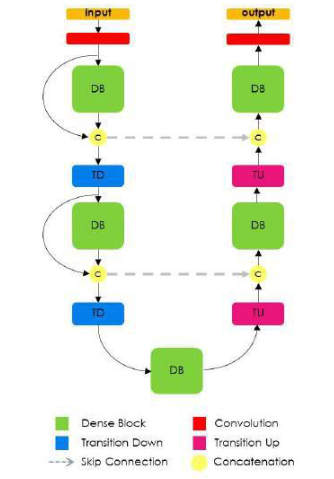
\includegraphics[width=.45\textwidth]{figures/tiramisu.png}
    \caption[Illustration of the fully convolution DenseNet.]{Illustration of the fully convolution DenseNet in \citep{jegou2017one}. The network consists of a downsampling path extracting high-level semantic features and an upsampling path recovering outputs to full resolution as input image. The skip connections, as indicated by dashed lines, combines both deep coarse features and shallow fine features.}
    \label{fig:tiramisu}
\end{figure}

The overall architecture of the network is depicted in Figure \ref{fig:tiramisu}, and how each component is structured is summarized in Table \ref{table:components}. For the network that we use in this thesis, it has 31 convolutional layers. Two max pooling layers are used to downsample the spatial size of inputs, and two deconvolution layers are used to recover outputs' resolution. Each dense block consists of 5 layers. One important parameter for dense block is the \textit{growth rate}, which is the number of feature maps in each layer. We use a growth rate of 12. Thus, the output of each dense block has $5 \times 12 = 60$ feature maps. The number of feature maps at the end of blocks is listed in Table \ref{table:number_feature_maps}. The network has in total 448,648 parameters.

\begin{table}[H]
\centering  
\begin{tabularx}{.9\textwidth}{c|c}
    \hline
    Component            & Structure            \\ \hline \hline
    Transition Down (TD) & BN $\rightarrow$ RELU $\rightarrow$ $1 \times 1$ CONV $\rightarrow$ $2 \times 2$ MAXPOOL \\ \hline
    Transition Up (TU)   & $3 \times 3$ DECONV with stride 2 \\
   \hline
   Layer                 & BN $\rightarrow$ RELU $\rightarrow$ $3 \times 3$ CONV \\ \hline
   Dense Block (DB).     & 5 Layers that are densely connected \\ \hline
  \end{tabularx}
\caption{Structure of each component in Figure \ref{fig:tiramisu}.}
\label{table:components}
\end{table}

\begin{table}[H]
\centering  
\begin{tabularx}{.45\textwidth}{c|c}
    \hline
    Order            & Number of feature maps            \\ \hline \hline
    Input                &    1 \\ \hline
    CONV                 &    8 \\ \hline
    DB + TD              &    68 \\ \hline
    DB + TD              &    128 \\ \hline
    DB                   &    60 \\ \hline
    TU + DB              &    188 \\ \hline
    TU + DB              &    60 \\ \hline
    CONV                 &    64 \\ \hline
    SOFTMAX              &    64 \\ \hline
  \end{tabularx}
\caption{Number of feature maps at the end of blocks.}
\label{table:number_feature_maps}
\end{table}

\section{Implementation of BOFMP} \label{sec:BOFMP_implementation}

Before tracking starts, the occupancy and velocity probabilities are initialized uniformly, i.e.,

\[ P_c\{ O = occ \}=P_c\{O = nocc\}=0.5  P_c\{V= v \}=1/number \ of \ velocities \] 

\section{Data Preprocessing}

\section{Hyperparameter Tuning} \label{sec:hyperparameter}

